The main requirements of the Vending Machine (VM):

\begin{enumerate}
\item The VM can sell one product, a coke-can.
\item When a sufficient amount of coins is inserted, one cocke-can will be dispensed from the VM.
\item The products price is fixed to 7 kr. ( in design this should be changeble )
\item The VM accepts 1 and 2 Kr coins.
\item A display should show the current total amount of money inserted.
\item A LED should indicate if change is avaliable (min 1 kr coin available).
\item Remove product sensor, will close the the coin slot and turn on indicating LED until product is removed.
\item Return Change.
\item Return all Coins.
\item If change is not available, the machine should only accept purchases with the right amount.
\end{enumerate}

\begin{figure}
\centering
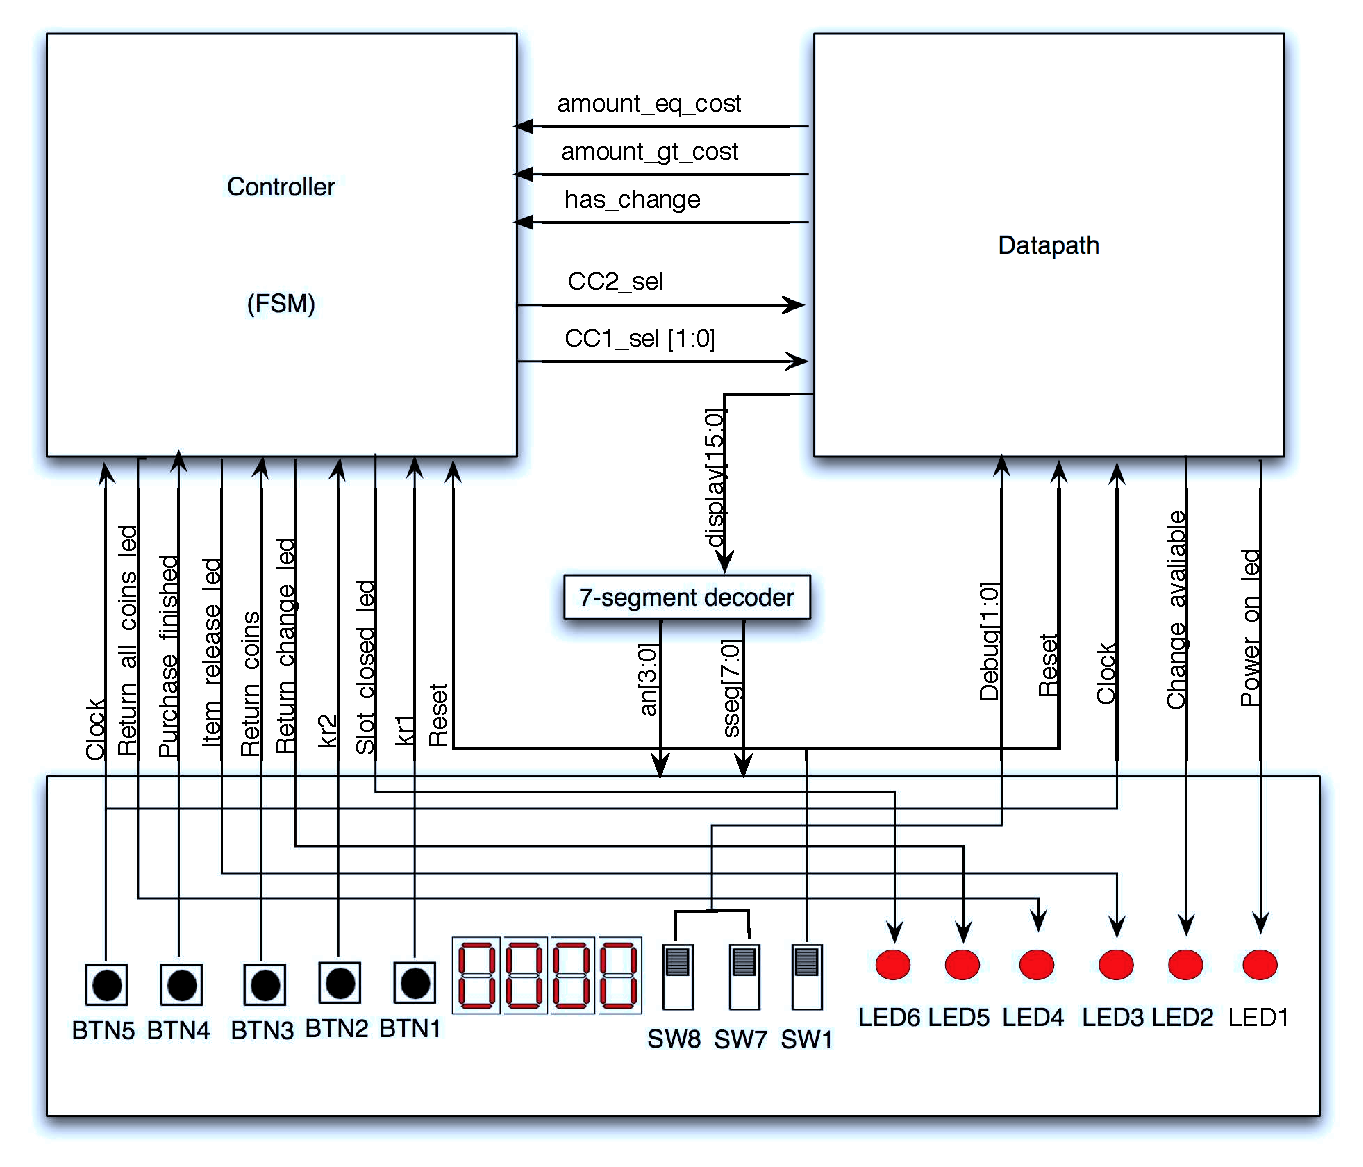
\includegraphics[width=0.8\textwidth]{fig/SystemDescription.pdf}
\caption{Overview of the processor}
\label{fig:system_description}
\end{figure}